\section[Phase de conception]{Phase de conception}
    \subsection[Diagramme de classes de conception]{Diagramme de classes de conception}
        \begin{figure}[H]
            \centering
            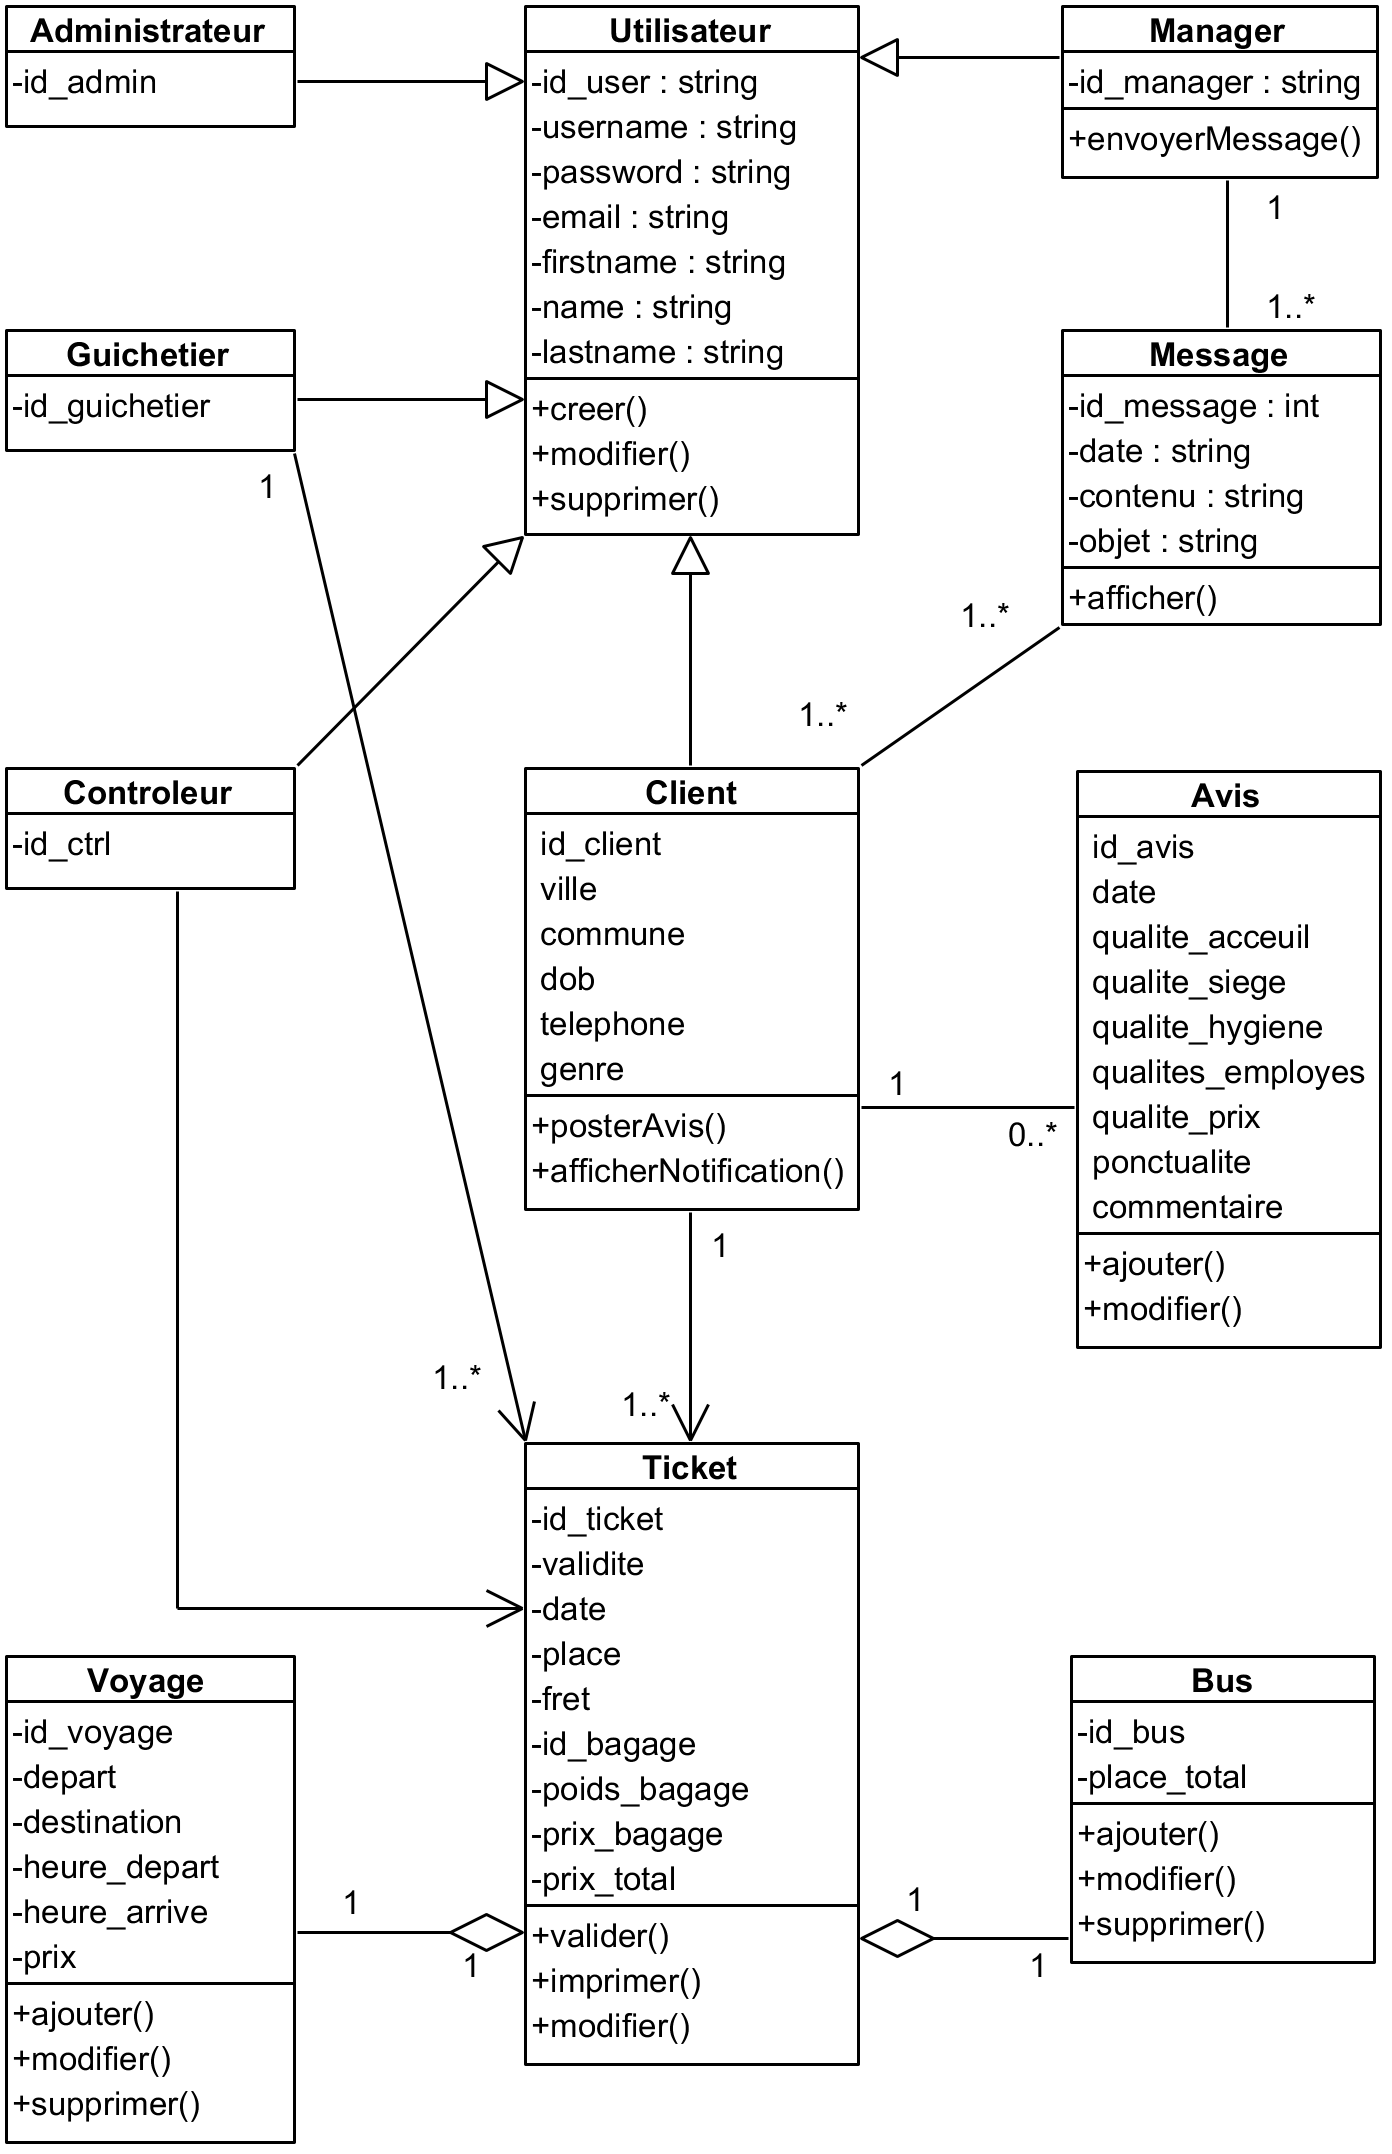
\includegraphics[width=130mm]{images/diagrammes-classe-de-conception/Classes de conception Class Diagram.png}
            \captionof{figure}{Diagramme de classes de conception}
            \label{fig:mdSysteme}
        \end{figure}
    \subsection[Diagramme de déploiement]{Diagramme de déploiement}
        \begin{figure}[H]
            \centering
            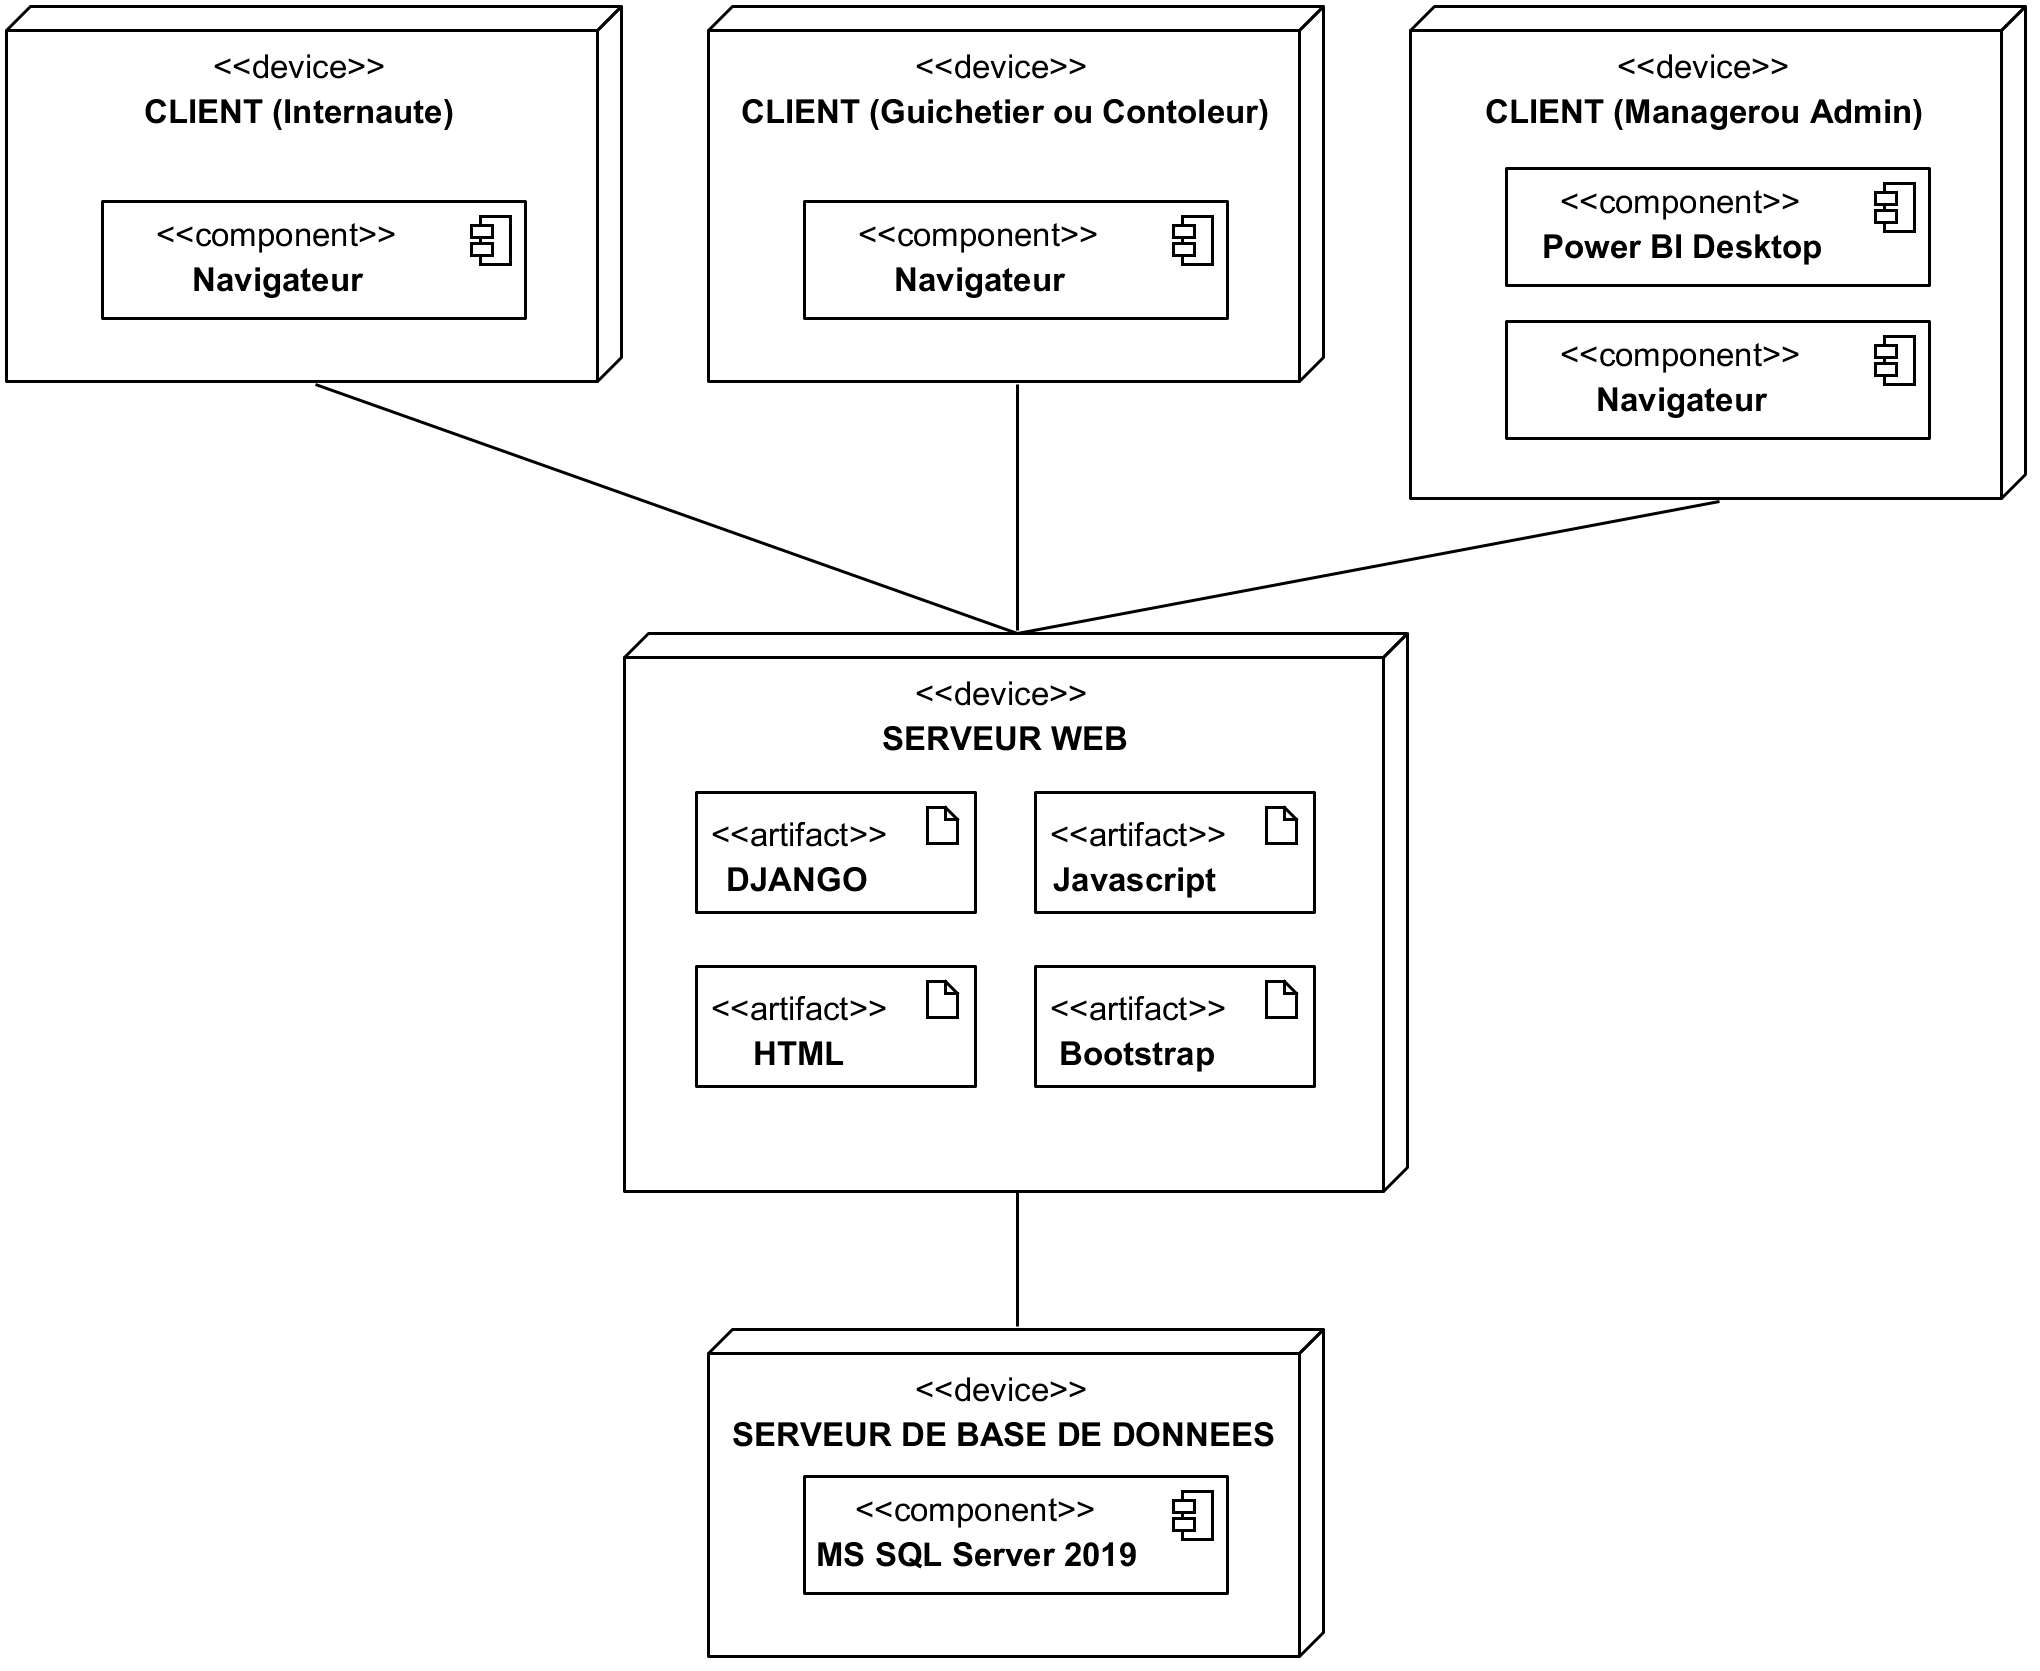
\includegraphics[width=150mm]{images/diagramme-de-deploiement/Diagramme de deploiement Deployment Diagram.png}
            \captionof{figure}{Diagramme de déploiement}
            \label{fig:diagDeploi}
        \end{figure}
    \subsection[Choix des indicateurs cles de performance (Démarche GIMSI)]{Choix des indicateurs clés de performance (Démarche GIMSI)}
    La qualité des décisions pouvant être prises est directement dépendante
    de la qualité de la mesure et de la pertinence des indicateurs choisis.
    \par
    Les indicateurs clés de performance de fidélisation client décrits
    ci-dessous, une fois insérés dans un tableau de bord élaboré avec soin,
    donneront une bien meilleure idée de la capacité à retenir le client et
    des axes d’amélioration à envisager. \cite*{JadeWin} :
    \par
    \begin{itemize}
        \setlength{\itemsep}{0pt}
        \item [\ding{226}] \textbf{Le Net Promoter Score} : correspond à
        la part de clients susceptibles de recommander, ou au contraire
        de déconseiller un produit, un service ou une marque.
        \item [\ding{226}] \textbf{Le taux d’attrition de la clientèle} : il sert à déterminer la proportion
        de clients perdus sur une période donnée.
        \item [\ding{226}] \textbf{Le taux satisfaction} : Il se base entièrement 
        sur l’évaluation de la satisfaction client qui a pour but de
        recueillir l’avis des clients sur les prestations délivrés, de repérer les
        insatisfactions et de réduire ceux que l’on juge préjudiciables
        à la bonne marche de l’activité.
    \end{itemize}
    \subsection[Modèle de l'entrepôt de données]{Modèle de l'entrepôt de données}
    Nous avons choisi un modèle en étoile pour notre entrepôt de données, il
    est présenté comme suite : 
        \begin{figure}[H]
            \centering
            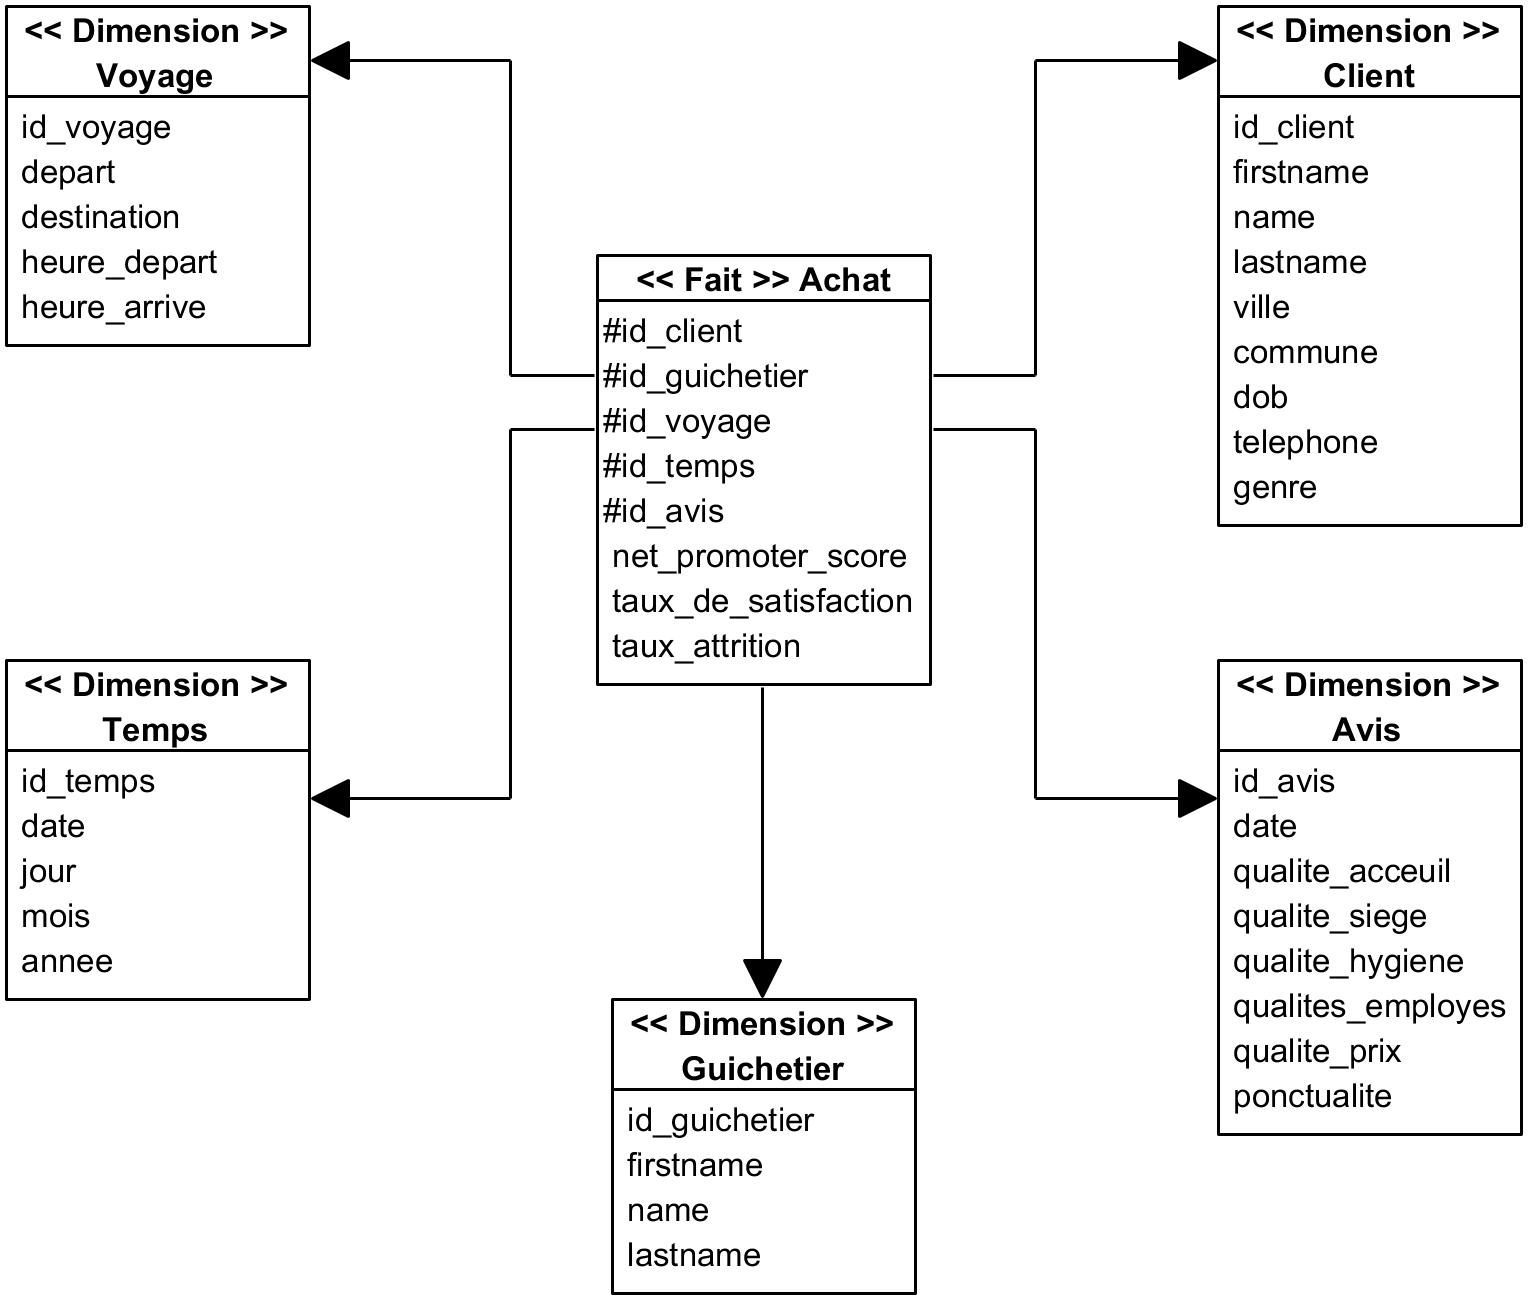
\includegraphics[width=150mm]{images/datawarehous-schema/Entrepot de donnees Class Diagram.png}
            \captionof{figure}{Modèle en étoile}
            \label{fig:dataWarehouse}
        \end{figure}